\chapter{Methodology}
In this chapter, we will first briefly summarize the KG extension and mining process, before exploring each component separately.

The process starts with a KG. From this KG we want to first mine rules, then extend it with new plausible facts, and lastly mine rules again on the extended KG. Candidates for additions to the KG are generated according to strategies that attempt to maximise the plausibility of the candidates. Once this set of candidate triples has been generated, the best of these are added to the KG. While there is no direct way to give an absolute score to these triples, a KG embedding trained on the original KG can rank the candidate triples against a set of corrupted triples. With the candidates ranked, one can accept all candidates above some appropriately chosen cutoff, and add them to the KG. Then rules can be mined and evaluated on both the original and extended KG, 
and results compared.
\begin{figure}[htp]
    \centering
    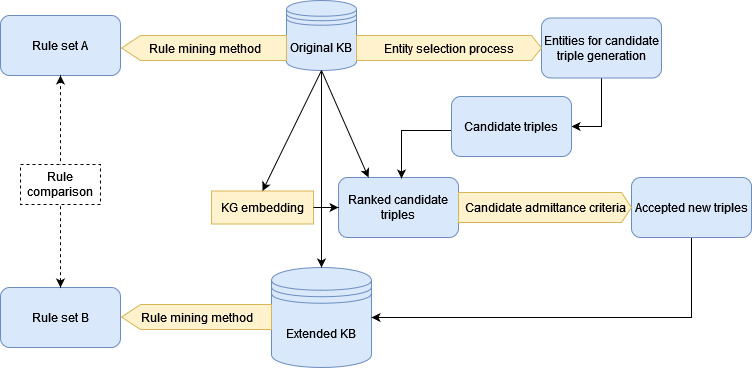
\includegraphics[width=16cm]{figures/ontology_mining_pipeline.jpg}
    \caption{Diagram representing KG extension and rule mining pipeline.}
\end{figure}

\section{Knowledge Graph Datasets}
While there are many large KGs publicly available, they are often quite complex in the number of different relations and entities used. Since we are mining rules over relations, the range of different relations was kept small. By restricting the number of relations, the resulting rules won't be overly diverse, and there will be many more candidate triples per relation when generating new plausible triples. Two different datasets were used to conduct the experiments, both of which were limited to contain only six different types of relations. We will discuss them next as we look at the KGs individually.


\subsection{Wikidata5M - family KG}
Wikidata5M is a KG dataset containing over 20 million triples with over 800 types of relations. It combines information from the Wikidata KG with Wikipedia pages \cite{wang2019kepler}. Wikidata5M uses the same identifier system as Wikidata, where each entity and relation is assigned a unique integer ID. The IDs of entities are prefixed with the letter \texttt{Q} and those of relations with \texttt{P}. For example the following line \\
\centerline{\texttt{\href{https://www.wikidata.org/wiki/Q146}{Q146} \quad \href{https://www.wikidata.org/wiki/Property:P279}{P279} \quad  \href{https://www.wikidata.org/wiki/Q39201}{Q39201}}} \
corresponds to \textless\texttt{\href{https://www.wikidata.org/wiki/Q146}{house cat}, \href{https://www.wikidata.org/wiki/Property:P279}{subclass of}, \href{https://www.wikidata.org/wiki/Q39201}{pet}}\textgreater, where each entity has a corresponding Wikipedia page.
This dataset was chosen due to its size and because it contained family-related information. Rules about family structure are well-known and easy to comprehend. For example the simple rule $parent(a, b) \Rightarrow  child(b, a)$ would be implicitly represented in the KG.
\begin{lstlisting}[float, language=Python, caption={Python dictionary converting family predicate IDs to their names.},captionpos=t, label={family_predicated_dict}]
family_predicates_dict = {
    'P40': 'child', 
    'P22' : 'father', 
    'P25' : 'mother',
    'P26' : 'spouse', 
    'P1038' : 'relative', 
    'P3373' : 'sibling', 
}
\end{lstlisting}

All triples that did not use one of the six selected family predicates were filtered out, and the IDs were converted to meaningful names so that the resulting rules mined would be easily readable. The python dictionary in \cref{family_predicated_dict} shows the chosen predicates. A few other family predicates were considered, but did not have enough corresponding data points or were too similar to other selected predicates. Common family-related predicates such as \texttt{grandchild} or \texttt{sister} are also not currently used in Wikidata. From a discussion in the Wikidata community it seems that all properties considered redundant were removed \cite{kinship_discussion}. Pykeen's distribution of the dataset was used for the experiments \cite{ali2021pykeen}. The resulting subset of Wikidata5M contained around 250 000 triples and will henceforth be referred to as the \textit{family KG}.

\subsection{WN18RR}
WN18RR is a smaller KG with 93 003 triples and only 11 relations \cite{dettmers2018convolutional}. It is an improved version of the WN18 dataset, where it was found that there was information leakage between the training and test set of WN18 through inverse relations. A large number of test triples could be identified simply by inverting triples in the training set \cite{toutanova2015observed}. For example the relation \texttt{has\_child} is the inverse relation of \texttt{has\_parent}, meaning that if the triple \texttt{(Ann, has\_parent, Carol)} is in the training set, then one can infer that \texttt{(Carol, has\_child, Ann)} likely is in the test set, thereby the test data is no longer consideres "unseen" not a fair data set to evaluate the model on. WN18RR addresses this issue. 

WN18RR contains triples scraped from WordNet, a lexical database for English \cite{wordNet}. In WordNet nouns, verbs, adjectives and adverbs are grouped into sets of semantic synonyms called
\textit{synsets} which express a distinct concept. For example \texttt{\{man\}} and \texttt{\{adult male\}} belong to the same synset. Synsets are connected to other synsets by semantic relations. The most commonly used relation in WN18RR is \texttt{hypernym}. A synset \texttt{X} is a hypernym of synset \texttt{Y}, if every \texttt{Y} is a kind of \texttt{X}. For example the triple 
\centerline{\texttt{02121808 \quad hypernym \quad 02121620}}
represents the information that the synset \texttt{cat} is a hypernym of the synset \texttt{house cat}. Or more simply phrased: \textit{All house cats are cats}.

\begin{table}[ht]
\centering
\begin{tabular}{|c|c|c|}
\hline
& \textbf{Relation} & \textbf{Frequency}\\
\hline
\multirow{6}{*}{\rotatebox[origin=c]{90}{Included}} &hypernym & 36873\\
&derivationally related form & 31865\\
&member meronym & 7912\\
&has part & 5131\\
&synset domain topic of & 3328\\
&instance hypernym & 3118\\
\hline
\multirow{5}{*}{\rotatebox[origin=c]{90}{Excluded}}&also see & 1396\\
&verb group & 1220\\
&member of domain region & 981\\
&member of domain usage & 673\\
&similar to & 86\\
\hline
\end{tabular}
\caption{Frequency of relations in WN18RR KG and whether they were included in the final KG.}
\end{table}

Though it is not vital for the reader to understand the semantics behind the relations in this dataset, it may be more rewarding to understand the terms when later reading rules mined from the WN18RR KG. The relation \texttt{hypernym} was described above, so now the remaining five relations are succintly explained.
\begin{itemize}
    \item \texttt{derivationally related form} \newline A concept $A$ derives from another concept $B$. \texttt{perfectly} is the derivationally related form of \texttt{perfect}.
    \item \texttt{member meronym}  \newline A concept $A$ is a member of a concept $B$. \texttt{class} is a member meronym of \texttt{student}.
    \item \texttt{has part} \newline A whole concept $A$ has a part $B$. \texttt{cat} has part \texttt{tail}.
    \item \texttt{synset domain topic of}  \newline A concept $A$ is the scientific field which concept $B$ belongs in. \texttt{computer science} is the synset domain topic of \texttt{deep learning}.
    \item \texttt{instance hypernym}  \newline denotes the type of an instance. \texttt{Bergen} has instance hypernym \texttt{city}.
\end{itemize}

WN18RR was chosen due to the few number of relations in it, and with a KG already containing few relations most of the data could be included.
By taking all triples containing one of the six most frequent relations, in total 88227 datapoints, 95\% of WN18RR was used. This was intended to produce a more complete KG. The dataset was loaded using AmpliGraph \cite{ampligraph}.

\section{Model selection}
There are many publicly available knowledge graph embedding libraries \cite{libkge, chandrahas-etal-2018-towards, ali2021pykeen}, but AmpliGraph's was chosen due to its thorough documentation and because it is an open source library based on Tensorflow, a well-known library for development of machine learning models \cite{tensorflow}. The library provides many different KG embedding models, performance metrics and KG datasets. Three different KG embedding methods were selected: TransE, DistMult and ComplEx. TransE was selected because it is one of the simplest and intuitive KG embedding models, but also it struggles with learning antisymmetric relationships, which are present in the KGs\footnote{In the family KG \textit{parent} and \textit{child} are antisymmetric relationships. In WN18RR \textit{hypernym} and \textit{derivationally related form} are antisymmetric relations.} (TODO: add source). So it most likely won't be a very good model for ranking candidate triples. (TODO: add justifications for DistMult and ComplEx after you have written about them in ch2) AmpliGraph also provides a baseline model, which the three selected models were compared to. The baseline model, called RandomBaseline, assigns a pseudo-random score to each triples it is asked to evaluate. When it comes to extending the KG this would essentially have the same effect as adding noise to the data.

Each model has a number of hyperparameters that could be optimised. As the search space grows it has been shown that random search is more optimal than grid search, where each combination needs to be tested \cite{bergstra2012random}. Due to limited computational resources, this approach to hyperparameter optimisation was selected. It is not an optimal approach, but serves as a practical and effective solution that measures well against more sophisticated methods such as Baysian optimisation \cite{li2017hyperband}.

\begin{table}[htbp]
\centering
\begin{tabular}{|l|l|}
\hline
\textbf{Hyperparameter}      & \textbf{Values}             \\ \hline
Batches count       & 50, 100                              \\ \hline
Epocs               & 50, 100                          \\ \hline
Embedding dimension                   & 50, 100, 200                     \\ \hline
$\eta$ (negative sampes @ rate)     & 5, 10, 15                            \\ \hline
Loss function   & pairwise, nll                         \\ \hline
Pairwise loss margin    & 0.5, 1, 2                    \\ \hline
%Regularizer         & LP                             \\ \hline
%Learning rate       & Random number in range(0.0001, 0.01) \\ \hline
\end{tabular}
%\label{{hyperparameter_table}
\caption{Hyperparameter values to search through in model selection.}
\end{table}
The AmpliGraph documentation was a main inspiration when deciding which hyperparameters to focus on. It was for example stated in the documentation that they received the best results with the adam optimizer, therefore other optimisers were not considered in the hyperparameter search \cite{ampligraph_documentation}. For each hyperparameter combination a learning rate randomly chosen in the range of 0.0001 - 0.01 was selected, another design choice borrowed from AmpliGraph.

For the implementation of model selection AmpliGraph's \texttt{select\_best\_mode\_ranking} was used. It is a model selection routine that allows for both grid and random search. At the end of each model selection process, the final model for each embedding type is retrained on the concatenation of the train and validation set, before it is eventually evaluated on the test set. The \texttt{eta} hyperparameter denotes the number of negative examples to be generated at training for each positive example, a process described in section (TODO: add section). % As the training data only contains positive examples, negative ones are generated.  In the training process corrupted triples are generated according to the strategy proposed by Bordes et al, which maintains the local closed world assumption \cite{TransE}.

\subsection{Model selection results}
The final model of all three embedding architectures had good results on the WN18RR dataset, and even better results on the family KG. Each model had an MRR score above 0.9 on the family KG and around 0.6 on the WN18RR. TransE seemed to perform slightly worse than DistMult and ComplEx on the family KG. On the WN18RR dataset TransE had a lower hits@1 score, while it outperformed both DistMult and ComplEx in both hits@3 and hits@10.
\begin{table}[htbp]
\centering
\begin{tabular}{|l||ccccc||ccccc|}
\hline
{\textbf{DATASET}}                 & \multicolumn{5}{c||}{\textbf{WN18RR}}                                                                                                                                               & \multicolumn{5}{c|}{\textbf{Family KG}}                                                                                                                            \\ \hline
\multirow{2}{*}{{\textbf{METRIC}}} & \multicolumn{1}{c|}{\multirow{2}{*}{\textbf{MR}}} & \multicolumn{1}{c|}{\multirow{2}{*}{\textbf{MRR}}} & \multicolumn{3}{c||}{\textbf{Hits@}}                                       & \multicolumn{1}{c|}{\multirow{2}{*}{\textbf{MR}}} & \multicolumn{1}{c|}{\multirow{2}{*}{\textbf{MRR}}} & \multicolumn{3}{c|}{\textbf{Hits@}}                                       \\ \cline{4-6} \cline{9-11} 
                                       & \multicolumn{1}{c|}{}                             & \multicolumn{1}{c|}{}                              & \multicolumn{1}{l|}{\textbf{1}} & \multicolumn{1}{l|}{\textbf{3}} & \multicolumn{1}{l||}{\textbf{10}} & \multicolumn{1}{c|}{}                             & \multicolumn{1}{c|}{}                              & \multicolumn{1}{l|}{\textbf{1}} & \multicolumn{1}{l|}{\textbf{3}} & \multicolumn{1}{l|}{\textbf{10}} \\ \hline
\textbf{Baseline}       & 495.32     & 0.007      & 0     & 0       & 0.01        & 498.72       & 0     & 0       & 0       & 0.1      \\ 
\textbf{TransE}  & 34.29  & 0.60       & 0.51                     & 0.66    & 0.76 & 2.59     & 0.93  &0.88  & 0.97   & 0.99   \\ 
\textbf{DistMult}      & 152.37  & 0.62    & 0.59   & 0.63      & 0.66   & 7.45    & 0.98     & 0.98    & 0.99   & 0.99    \\ 
\textbf{ComplEx}        & 139.36    & 0.59      & 0.57      & 0.60      & 0.63      & 4.64     & 0.99     & 0.98     & 0.99      & 0.99  \\ \hline
\end{tabular}
\caption{Results of selected models evaluated on test set.}
\end{table}


\begin{figure}[htbp]
\centering
\begin{subfigure}{.5\textwidth}
  \centering
  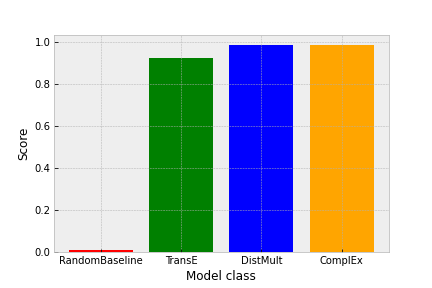
\includegraphics[width=1\linewidth]{figures/model_selection/family_mrr.png}
  \caption{MRR scores}
  \label{fig:model_selection_mrr_family}
\end{subfigure}%
\begin{subfigure}{.5\textwidth}
  \centering
  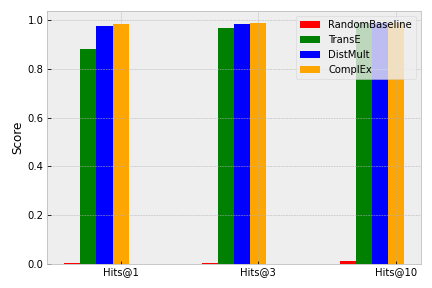
\includegraphics[width=1\linewidth]{figures/model_selection/family_hit_scores.png}
  \caption{Hits@n scores}
  \label{fig:model_selection_hit_scores_family}
\end{subfigure}
\caption{KG embedding test performance results for Wikidata5M (family KG).}
\label{fig:model_selection_metrics_family}
\end{figure}

\begin{figure}[htbp]
\centering
\begin{subfigure}{.5\textwidth}
  \centering
  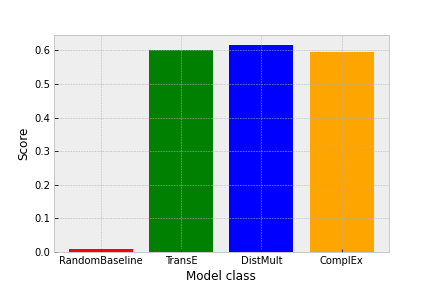
\includegraphics[width=1\linewidth]{figures/model_selection/wn18rr_mrr.png}
  \caption{MRR scores}
  \label{fig:model_selection_mrr_wn18rr}
\end{subfigure}%
\begin{subfigure}{.5\textwidth}
  \centering
  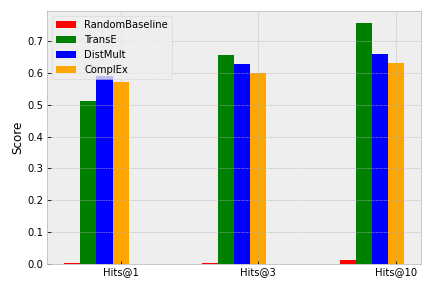
\includegraphics[width=1\linewidth]{figures/model_selection/wn18rr_hit_scores.png}
  \caption{Hits@n scores}
  \label{fig:model_selection_hit_scores_wn18rr}
\end{subfigure}
\caption{KG embedding test performance results for WN18RR}
\label{fig:model_selection_metrics_wn18rr}
\end{figure}


%epochs (int) – The iterations of the training loop.

%batches_count (int) – The number of batches in which the training set must be split during the training loop.

%k (int) – Embedding space dimensionality.

%loss : pairwise loss, with a margin of 0.5 set via the loss_params kwarg.

\newpage

\section{KG extension}

The goal of KG extension is to add potentially true statements to the original KG. AmpliGraph does have an implementation for this, called \texttt{discover\_facts}, but due to computational limitations\footnote{\texttt{discover\_facts} uses \textit{all} entities in the KG to generate counterexamples. In large KGs like the ones used in our experiments, this is not feasible.} it could not be used.
The implementation used in this thesis does however follow the same general strategy used in \texttt{discover\_facts}. It consists of two main components:
\begin{enumerate}
    \item Candidate triple generation
    \item Ranking of generated candidates
\end{enumerate}
With a set of ranked candidate triples all that remains is to decide what the minimum rank should be for a candidate to be admitted to the KG.


\subsection{Candidate triple generation}
\label{canidate_triple_generation}
Both in the family KG and in WN18RR the number of potential facts is huge, and so in order to avoid having to evaluate all of them a number of strategies can be used to select plausible facts. In AmpliGraph's implementation of plausible candidate generation, they make the assumption that densely connected entities are less likely to have missing true statements. In a KG embedding tutorial at the European Conference on Artificial Intelligence in 2020, members of the AmpliGraph team say that this assumption has been true for their empirical evaluations, but is not necessarily true for all datasets \cite{kge_tutorial}.  As stated, AmpliGraph has implemented different strategies, many of which have to do with graph clustering, but these were too computationally intensive to take into use. Four simpler strategies for entity selection were instead used:
\begin{itemize}
    \item Random selection of entities.
    \item Selecting the most frequent entities.
    \item Selecting the least frequent entities.
    \item Probabilistic selection based on the frequency of the entities in the dataset, where the least frequent entities are most likely to be selected.
\end{itemize}

\begin{table}[htbp]
\centering
\begin{tabular}{rcl|lcc}
\multicolumn{3}{c|}{\textbf{KG}}                    &  & \multicolumn{1}{l}{\textbf{Entity}} & \multicolumn{1}{l}{\textbf{Freq.}} \\\hline
\textit{Ann} & \textit{sibling} & \textit{Bob}   &  & Ann                               & 4                                      \\
\textit{Ann} & \textit{sibling} & \textit{Carl} &  & Bob                                 & 3                                      \\
\textit{Ann} & \textit{friend}  & \textit{Carl} &  & Carl                               & 3                                      \\
\textit{Bob}   & \textit{friend}  & \textit{Carl} &  & Dave                                & 2                                      \\
\textit{Bob}   & \textit{friend}  & \textit{Dave}  &  & Eve                                 & 2                                      \\
\textit{Ann} & \textit{friend}  & \textit{Eve}   &  & Felix                               & 1                                      \\
\textit{Felix} & \textit{friend}  & \textit{Gina}  &  & Gina                                & 1                                      \\
\textit{Dave}  & \textit{friend}  & \textit{Eve}   &  & \multicolumn{1}{l}{}                & \multicolumn{1}{l}{}                  
\end{tabular}
\label{entity_selection_KG}
\caption{Example KG with frequency table of entities.}
\end{table}

If we look at \cref{entity_selection_KG} as an example KG and need to select three entities for candidate generate, then with the 
\begin{itemize}
    \item \textit{most frequent} strategy the entity set would be \{\textit{Ann, Bob, Carl}\},
    \item \textit{least frequent} strategy the entity set would be \{\textit{Dave, Felix, Gina}\},
    \item \textit{probabilistic} strategy the entity set could be \{\textit{Gina, Eve, Felix}\},
\end{itemize}
and any three candidates would be selected with the \textit{random} strategy. Note that selection is without replacement. Once the entities were selected, all possible triples were generated with them and the six relations. Then, all the triples already included in the original KG were excluded from the resulting candidate triples. If one were to pick the \textit{most frequent} strategy, then the resulting set of candidate triples would be that depicted in \cref{canidate_triples_most_frequent}. Of course the more candidate triples there are to choose from, the better the extension will be because then there is a higher chance of plausible facts being suggested. Again, computational limitations restricted this. After trying different candidate set sizes it was eventually decided that selecting 1000 entities for candidate triple generation was a feasible number. This meant that $ 1000 \times 6 \times 1000 = 6 \times 10^6 $ triples (minus those that already appeared in the KG) were considered for each KG extension.


\begin{table}[htbp]
\centering
\begin{tabular}{rcllrcl}
\multicolumn{7}{c}{\textbf{Candiate Triples}}                                                                                                                                                                                                       \\
\textit{Ann}                        & \textit{sibling}                        & \textit{Ann}                        &  & \textit{Ann}                        & \textit{friend}                        & \textit{Ann}                        \\
{\color[HTML]{CB0000} \textit{Ann}} & {\color[HTML]{CB0000} \textit{sibling}} & {\color[HTML]{CB0000} \textit{Bob}}   &  & \textit{Ann}                        & \textit{friend}                        & \textit{Bob}                          \\
{\color[HTML]{CB0000} \textit{Ann}} & {\color[HTML]{CB0000} \textit{sibling}} & {\color[HTML]{CB0000} \textit{Carl}} &  & {\color[HTML]{CB0000} \textit{Ann}} & {\color[HTML]{CB0000} \textit{friend}} & {\color[HTML]{CB0000} \textit{Carl}} \\
\textit{Bob}                          & \textit{sibling}                        & \textit{Ann}                        &  & \textit{Bob}                          & \textit{friend}                        & \textit{Ann}                        \\
\textit{Bob}                          & \textit{sibling}                        & \textit{Bob}                          &  & \textit{Bob}                          & \textit{friend}                        & \textit{Bob}                          \\
\textit{Bob}                          & \textit{sibling}                        & \textit{Carl}                        &  & {\color[HTML]{CB0000} \textit{Bob}}   & {\color[HTML]{CB0000} \textit{friend}} & {\color[HTML]{CB0000} \textit{Carl}} \\
\textit{Carl}                        & \textit{sibling}                        & \textit{Ann}                        &  & \textit{Carl}                        & \textit{friend}                        & \textit{Ann}                        \\
\textit{Carl}                        & \textit{sibling}                        & \textit{Bob}                          &  & \textit{Carl}                        & \textit{friend}                        & \textit{Bob}                          \\
\textit{Carl}                        & \textit{sibling}                        & \textit{Carl}                        &  & \textit{Carl}                        & \textit{friend}                        & \textit{Carl}                       
\end{tabular}
\caption{Candidate triples for \cref{entity_selection_KG} KG, using entity selection method \textit{most frequent}, and entity set size 3. Triples in red are already present in the KG, and are removed from the candidates set.}
\label{canidate_triples_most_frequent}
\end{table}


\subsection{Candidate triple ranking}
As discussed in Section \ref{Performance_indicators}, it is not easy to set an absolute score to a triple with a KG embedding. Therefore candidate triples are instead ranked against corrupted triples. An accurate KG embedding model will rank well-suited candidates higher than the corrupted triples. Since only one side of each triple is corrupted at a time, the corrupted triples generated are compliant with the local closed world assumption. AmpliGraph's function \texttt{evaluate\_performance} evaluates the performance of a trained KG embedding model by ranking a set of test triples from the KG against a set of corrupted triples. An embedding model is then evaluated based on how good it is at ranking the positive test triples higher than the negative corrupted triples. By instead passing the set of candidate triples to \texttt{evaluate\_performance} these could be ranked instead. Once the candidates have been given ranks one simply needs to decide on a cutoff rank to consider the candidate as a true fact and add it to the KG. The rank cutoffs that were considered were 1, 4 and 7. These values were chosen as they are in the range of typical Hits@K cutoff values. Rank cutoff 1 is the strictest cutoff possible where only candidates ranked higher than \textit{all} the corrupted triples are admitted. Hits@1 is also the strictest Hit ratio performance metric, where the triple with highest score must be a true fact in the KG. As stated in Section \ref{Hits@k}, hit ratio cutoff values larger than 10 are rarely used. Therefore other two rank cutoff values within this range were chosen.

\section{Rule mining and evaluation}
Rules are mined using the rule mining algorithm AMIE3 \cite{amie3}. The authors of AMIE3 have made an implementation of it available on \hyperlink{https://github.com/lajus/amie}{GitHub}. It is released as a executable jar file that takes a KG in TSV file format as input and outputs rules accompanied with various confidence scores. The jar file in release 3.0 was used for rule mining. It was run using the default settings used in the AMIE3 paper by Lajus et al \cite{amie3}. Since default settings change, the exact command used for rule mining was: \texttt{java -jar amie-milestone-intKB.jar -bias lazy -full -noHeuristics -ostd [TSV file]}.

As previously mentioned, the implementation of AMIE3 outputs the rules accompanied with confidence scores. Unfortunately the scores are calculated on the same dataset on which the rules have been mined on. Since these datasets have been extended they may contain datapoints that are false positives, leading to evaluation based on erroneous data. New rules that follow this incorrect data will therefore possibly receive high scores despite not making sense in the given context. To amend this problem all mined rules are also evaluated on the original KG.
% Jørn: Is the following paragraph relevant? no.
This was not previously available in any release of AMIE3, which only allows rule evaluation in combination with rule mining, on the dataset from which the rules are being mined. Evaluation of rules on a custom KG was not possible until one of the authors, Jonathan Lajus, was kind enough to add a script to do exactly this.

In the final results from the experiments run, each mined rule had two different sets of confidence scores, one evaluated on the original KG and the other on the extended KG. In addition to scores, each rule was also accompanied by the parameters under which the KG was extended. These three parameters are the \textit{entity selection method}, the \textit{KG embedding model} used to rank candidates and the \textit{rank cutoff value} for candidate admittance. In summary, the output data points in the rule mining and evaluation process had these features:
\begin{itemize}
    \item Rule
    \item Metrics
        \subitem Head Coverage (extended and original KG)
        \subitem PCA Confidence (extended and original KG)
        \subitem Positive Examples (extended and original KG)
        \subitem PCA body size (extended and original KG)
    \item Parameters
        \subitem Entity seleciton method
        \subitem KG embedding model
        \subitem Rank cutoff
    \item Boolean indication for whether rule was also mined from the original KG
\end{itemize}

With this information one can look at the effect the parameters have on the number of rules mined and how the measured confidence differs when calculated on the extended KG versus the original KG.


\section{Additional experimental setup details}
The experiments were run on a server with 64 GB of RAM and an Intel Core i9-7900X 3.3GHz processor.

The implementation of AMIE used in this thesis is distributed under the \hyperlink{https://creativecommons.org/licenses/by-nc/3.0/}{Creative Commons Attribution-NonComercial license v3.0} by the \hyperlink{https://www.mpi-inf.mpg.de/departments/databases-and-information-systems/research/yago-naga/amie/}{YAGO-NAGA team} and the \hyperlink{https://dig.telecom-paris.fr/blog/}{DIG team}. The program uses Javatools, a library released under the \hyperlink{https://creativecommons.org/licenses/by/3.0/}{Creative Commons Attribution license v3.0} by the \hyperlink{https://www.mpi-inf.mpg.de/departments/databases-and-information-systems/research/yago-naga/amie/}{YAGO-NAGA team}.
